\section{Experiment}
\label{sec:experiment}

\subsection{Feature Engineering}
\label{sub:feature_engineering}

\subsubsection{Sequence Smoothing}
\label{ssub:sequence_smoothing}

\begin{figure}[htpb]
   \centering
   \subfloat[Send gaps]{
      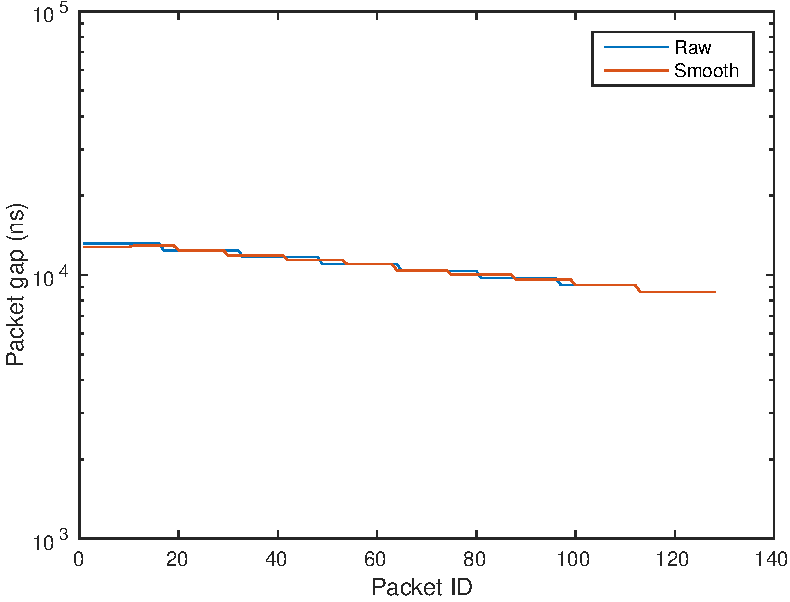
\includegraphics[width=0.45\linewidth]{figures/smooth_send.pdf}
   }
   \quad
   \subfloat[Received gaps]{
      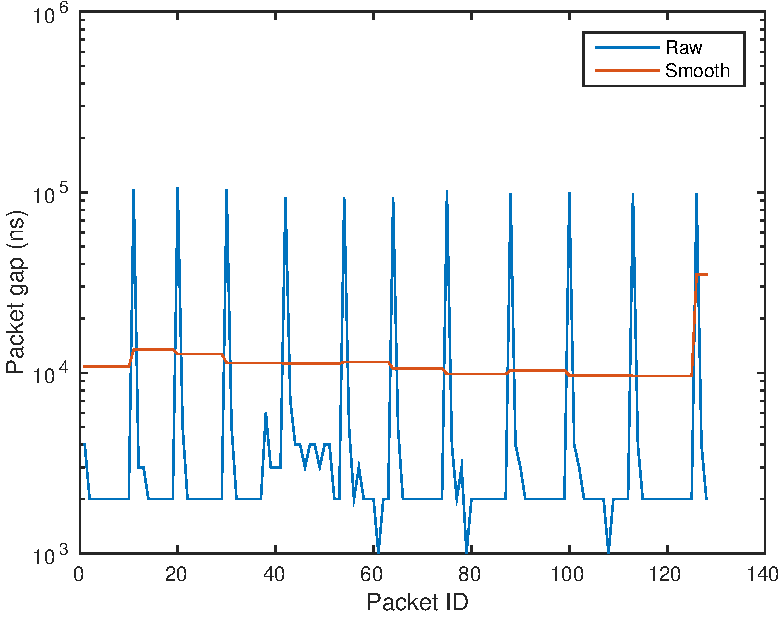
\includegraphics[width=0.45\linewidth]{figures/smooth_recv.pdf}
   }
   \caption{Smoothing raw packet gaps.}
   \label{fig:smoothing}
\end{figure}

\subsubsection{Fourier Transformation}
\label{ssub:fourier_transformation}

\begin{figure}[htpb]
   \centering
   \subfloat[Send gaps]{
      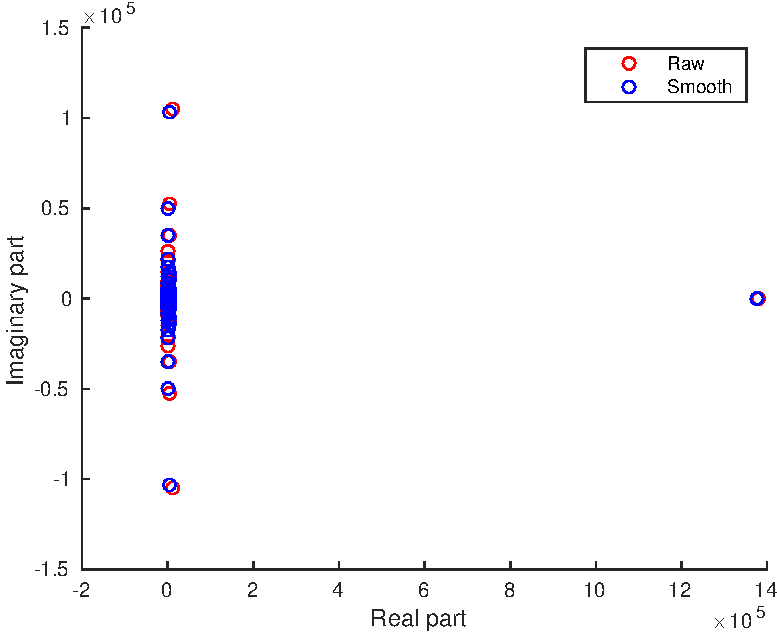
\includegraphics[width=0.45\linewidth]{figures/fft_send.pdf}
   }
   \quad
   \subfloat[Received gaps]{
      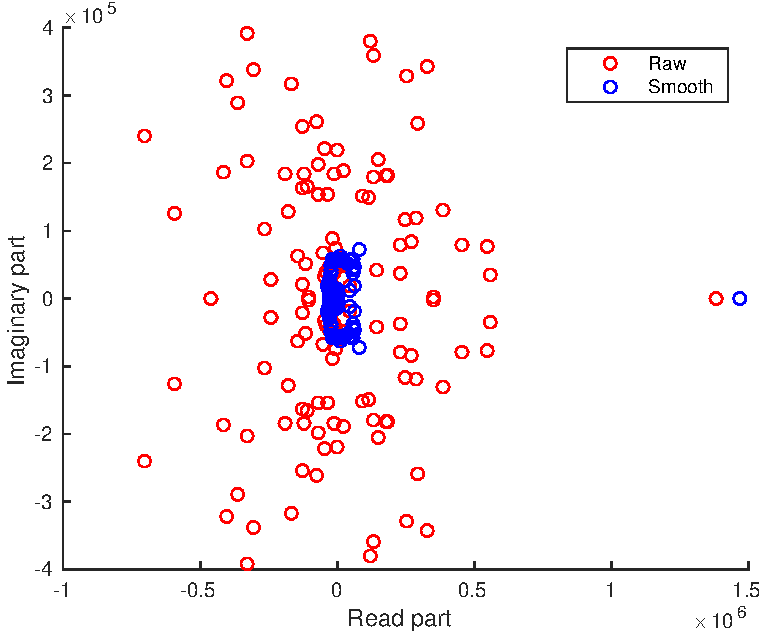
\includegraphics[width=0.45\linewidth]{figures/fft_recv.pdf}
   }
   \caption{Fourier transformation on raw packet gaps.}
   \label{fig:fft}
\end{figure}

\subsection{Experimental Setting}
\label{sub:parameter_setting}

We collected data using the experimental setting in \cite{Yin2014} and has the
following datasets for our evaluation. We discarded incomplete streams. And for
cases where we don't have baseline prediction from \cite{Yin2014} we cannot do
a fair comparison, we discarded such stream. Detailed statistics of datasets
can be found in Table~\ref{tab:dataset}.

\begin{table}[htpb]
   \centering
   \caption{Dataset}
   \label{tab:dataset}
   \begin{tabular}{|c|c|c|c|c|l|l|l|l|}
      \hline
      Name & Range & Rate & Packets & Length & Total & Valid          & Training & Test\\ \hline
      Exp4 & 50    & 8    & 16      & 128    & 11003 & 7475(67.94\%)  & 5233     & 2242 \\
      Exp5 & 50    & 2    & 16      & 128    & 11003 & 7188(65.33\%)  & 5032     & 2156 \\
      Exp6 & 50    & 3    & 16      & 129    & 10691 & 883(8.26\%)    & 618      & 265 \\
      Exp7 & 50    & 6    & 16      & 126    & 11016 & 7203(65.39\%)  & 5042     & 2161 \\
      Exp8 & 50    & 4    & 16      & 128    & 33310 & 18185(54.59\%) & 12730    & 5455  \\ \hline
   \end{tabular}
\end{table}

In order to achieve better performance, we ran a 5 fold cross validation on the
training dataset to tune parameters of different estimators. Here are the
parameter settings we use for prediction:
\begin{itemize}
   \item AdaBoost: we used 200 decision tree regressor as base estimators. With
      learning rate of 1.0, and linear loss function, we acheived an error rate
      of 2.18\%.
   \item Elastic net: we used a smaller learning rate $\alpha=0.5$, together
      with a $L_1$ ratio $\rho=0.5$. Optimization by coordinate descent can
      converage within 50000 iterations with a threshold of $0.3$.
   \item Gradient boost: we used least squares regression as the loss function,
      with learning rate of $0.1$, 200 boosting stages. For each individual
      regression estimator, we constrain the maximum depth to be 3, minimum
      number of samples of spliting internal node to be 2, minimum number of
      samples required to be a leaf node to be 2.
   \item Lasso: we adopted a higher learning rate of $\alpha=1$. Optimization
      by coordinate descent can converage within 10000 iterations with a
      threshold of $0.5$. With such a relatively high threshold, we can still
      achieve an average error rate of $2.03\%$.
   \item Nearest neighbor regression: we used a fix number of 10 nearest
      neighbors for the regression. Neighboring data points are weighted by
      the inverse of the distance to the query data point. In order to speed up
      searching, we adopted KD-tree as the underlying structure. Leaf node size
      is set to 30. Euclidean distance is used as distance metric.
   \item Random forest regressor: we used 10 trees to assemble the random
      forest. Mean squared error is used as the split quality measure. Minimum
      number of samples required to split an internal node is set to 2, minimum
      number of samples in newly created leaves is set to 1.
\end{itemize}

\subsection{Benchmark}
\label{sub:benchmark}

\subsubsection{Computation Performance}
\label{ssub:computation_performance}



\begin{table}[htpb]
   \centering
   \caption{Average processing time over 28655 streams.}
   \label{tab:timing}
   \begin{tabular}{|c|r|r|r|r|r|r|}
      \hline
      \multirow{2}{*}{Algorithms} & \multicolumn{2}{c|}{Feature extraction} &
      \multicolumn{4}{c|}{Training} \\ \cline{2-7}
                       & Raw   & Smooth & Raw            & Raw FFT        & Smooth         & Smooth FFT \\ \hline
      AdaBoost         & 15.71 & 14.94  & 2026.13        & 35766.15       & 13109.74       & 32991.03\\
      Elastic net      & 16.60 & 16.06  & 151.96         & 577.30         & 121.73         & 537.47\\
      Gradient boost   & 12.55 & 12.52  & 8090.82        & 45908.08       & 9695.63        & 46406.90\\
      Lasso            & 16.23 & 16.14  & 145.09         & 507.52         & 139.83         & 567.07\\
      NNR              & 15.78 & 15.59  & \textbf{18.75} & \textbf{33.29} & \textbf{18.34} & \textbf{35.41}\\
      Random forest    & 15.80 & 15.61  & 3139.64        & 9236.24        & 3207.93        & 9380.83\\
      \hline
   \end{tabular}
\end{table}

\subsubsection{Accuracy}
\label{ssub:accuracy}
\begin{table}[htpb]
   \centering
   %6.97
   \caption{Average accuracy of different estimators over differnt features. We
      evaluated the average accuracy over all test datasets, with 12279 probing
      sequences in total. We include accuracy increases compared with baseline
      from \cite{Yin2014} in parentheses. \cite{Yin2014} has an average
      accuracy of 6.97\%.}
   \label{tab:accuracy}
   \begin{tabular}{|c|c|c|c|c|}
      \hline
      Algorithms     & Raw                      & Raw FFT                  & Smooth                   & Smooth FFT \\ \hline
      AdaBoost       & 2.82\%(59.43\%)          & 2.38\%(65.72\%)          & 2.29\%(67.14\%)          & 2.18\%(68.65\%)\\
      Elastic net    & 2.30\%(66.95\%)          & 2.19\%(68.58\%)          & 2.16\%(68.97\%)          & 1.96\%(71.87\%)\\
      Gradient boost & 2.41\%(65.34\%)          & \textbf{1.96\%}(71.75\%) & \textbf{1.89\%}(72.88\%) & \textbf{1.82\%}(73.77\%)\\
      Lasso          & 2.70\%(61.18\%)          & 2.37\%(65.89\%)          & 2.25\%(67.65\%)          & 2.03\%(70.78\%)\\
      NNR            & \textbf{2.29\%}(67.11\%) & 2.29\%(67.11\%)          & 2.17\%(68.83\%)          & 2.17\%(68.83\%)\\
      Random forest  & 2.35\%(66.26\%)          & 2.01\%(71.06\%)          & 2.05\%(70.47\%)          & 1.89\%(72.86\%)\\
      \hline
   \end{tabular}
\end{table}

\begin{figure}[htpb]
   \centering

   \subfloat[AdaBoost]{
      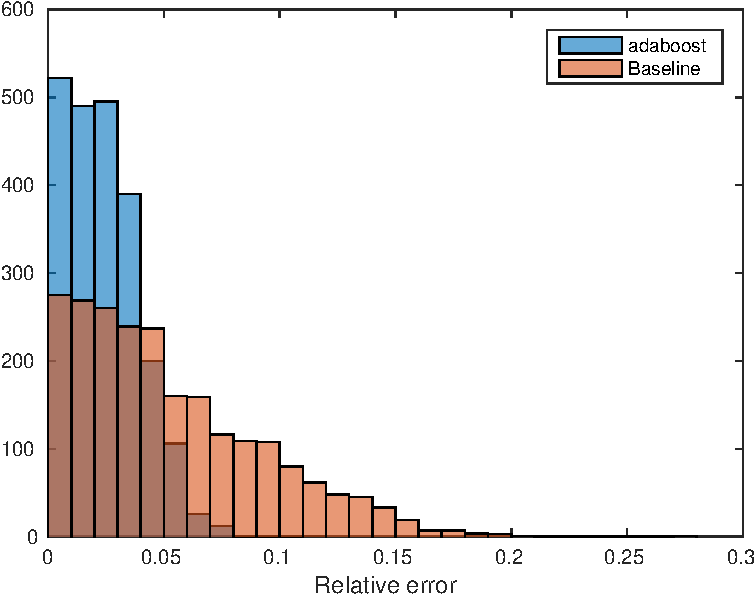
\includegraphics[width=0.3\linewidth]{figures/histogram_adaboost.pdf}
   }
   \quad
   \subfloat[Elastic net]{
      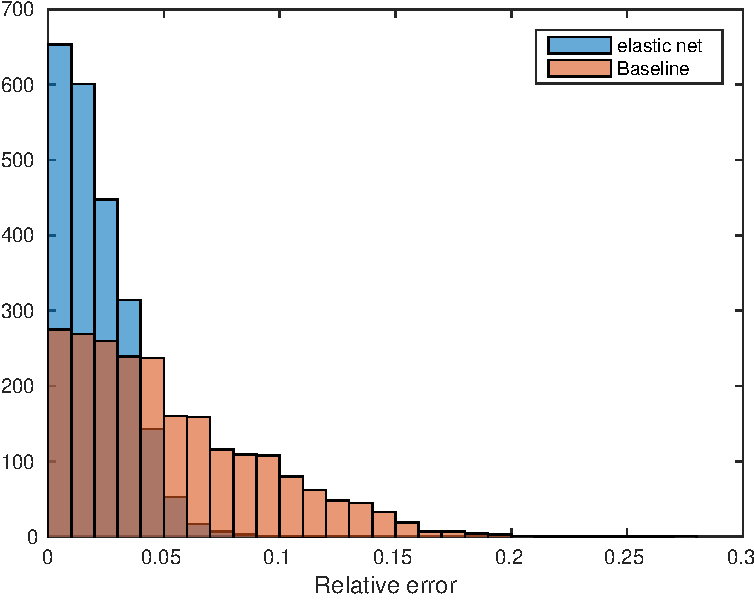
\includegraphics[width=0.3\linewidth]{figures/histogram_elastic_net.pdf}
   }
   \quad
   \subfloat[Gradient boost]{
      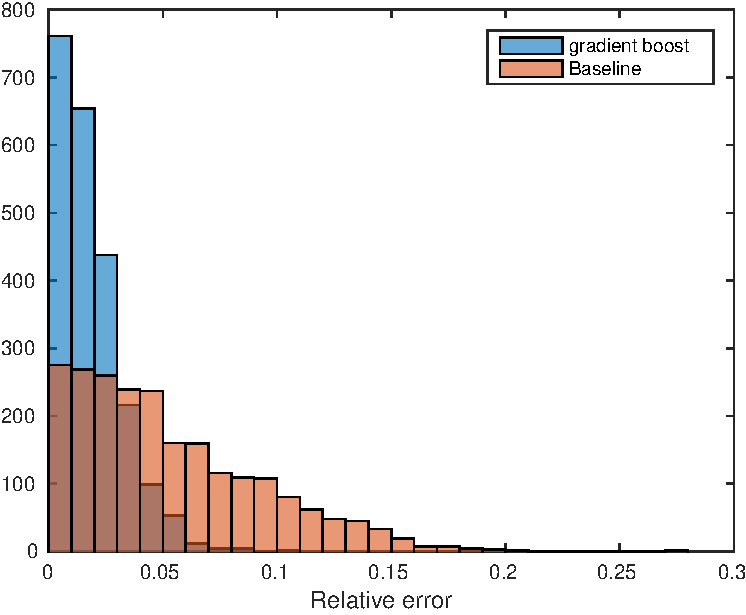
\includegraphics[width=0.3\linewidth]{figures/histogram_gradient_boost.pdf}
   }
   \\
   \subfloat[Lasso]{
      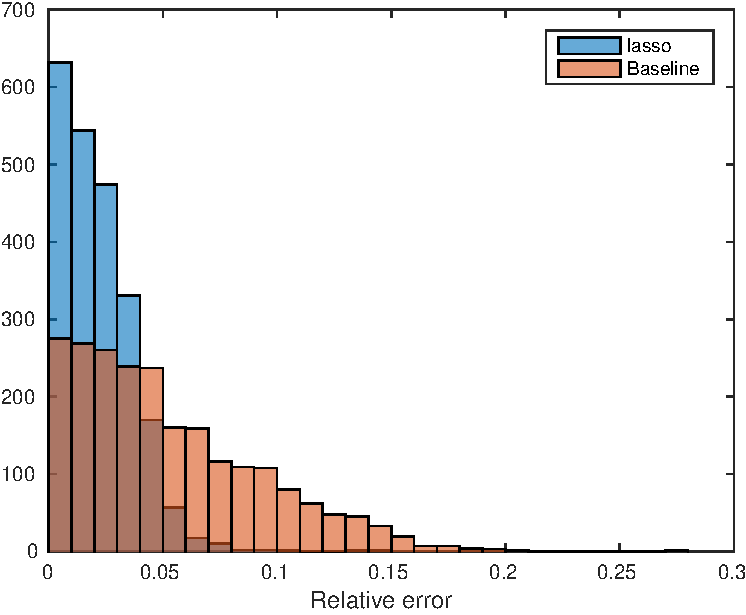
\includegraphics[width=0.3\linewidth]{figures/histogram_lasso.pdf}
   }
   \quad
   \subfloat[NNR]{
      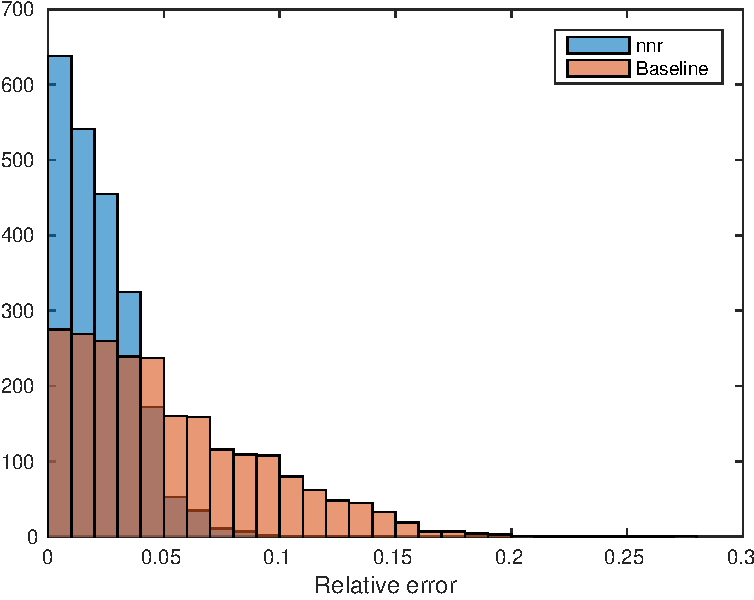
\includegraphics[width=0.3\linewidth]{figures/histogram_nnr.pdf}
   }
   \quad
   \subfloat[Random forest]{
      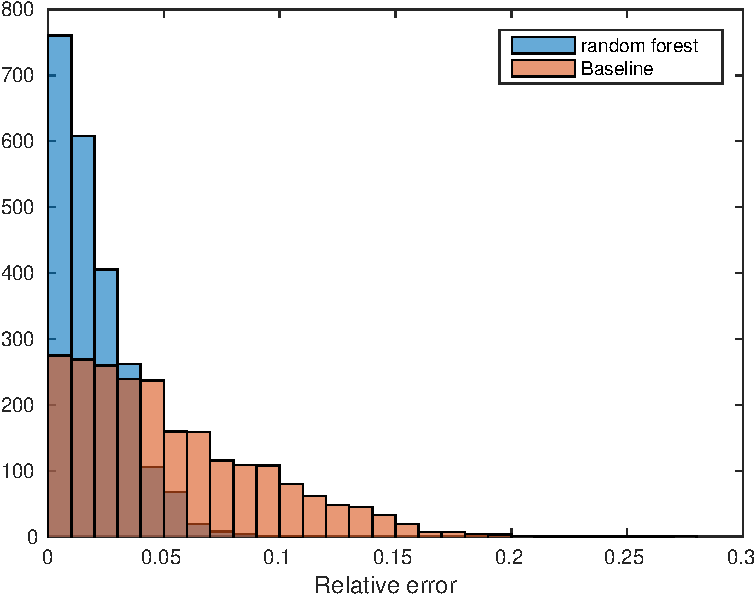
\includegraphics[width=0.3\linewidth]{figures/histogram_random_forest.pdf}
   }
   \caption{Relative error histograms of different estimators. We ran learning
      based estimators on FFT transformed smooth sequences. Example dataset has
      range 50, rates 8, packets 16.}
   \label{fig:name}
\end{figure}

\begin{figure}[htpb]
   \centering
   \subfloat[Relative error]{
      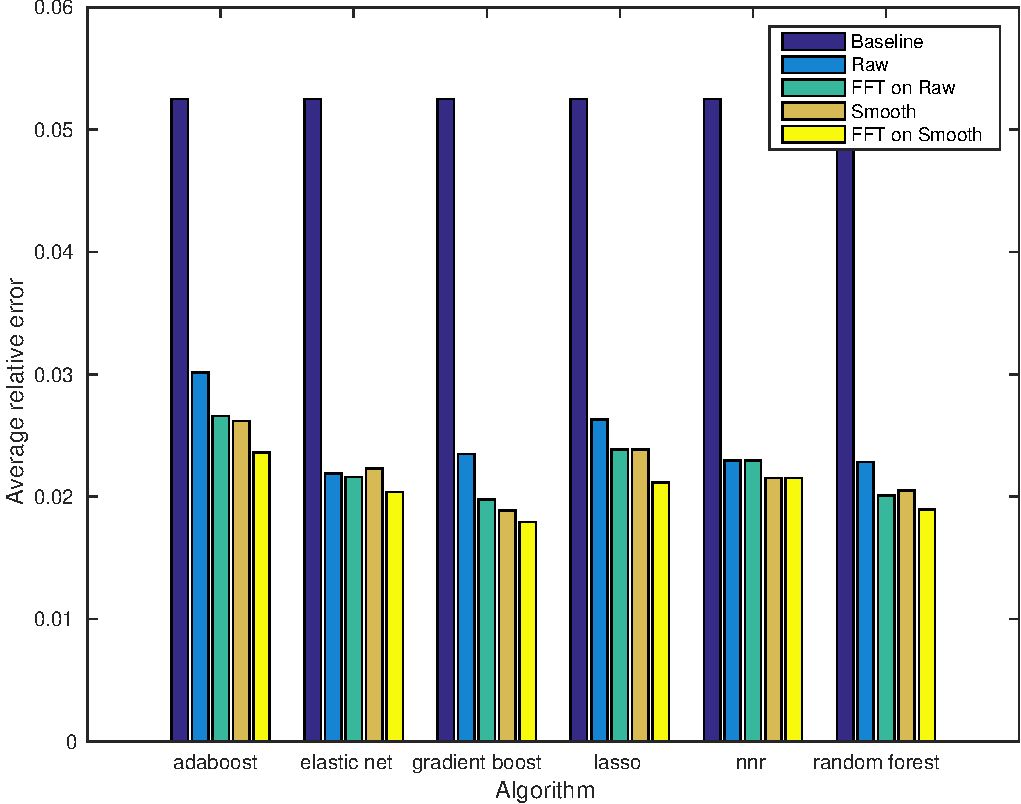
\includegraphics[width=0.45\linewidth]{figures/error_exp4_range50_rates8_pkts16.pdf}
   }
   \quad
   \subfloat[Standard derivation]{
      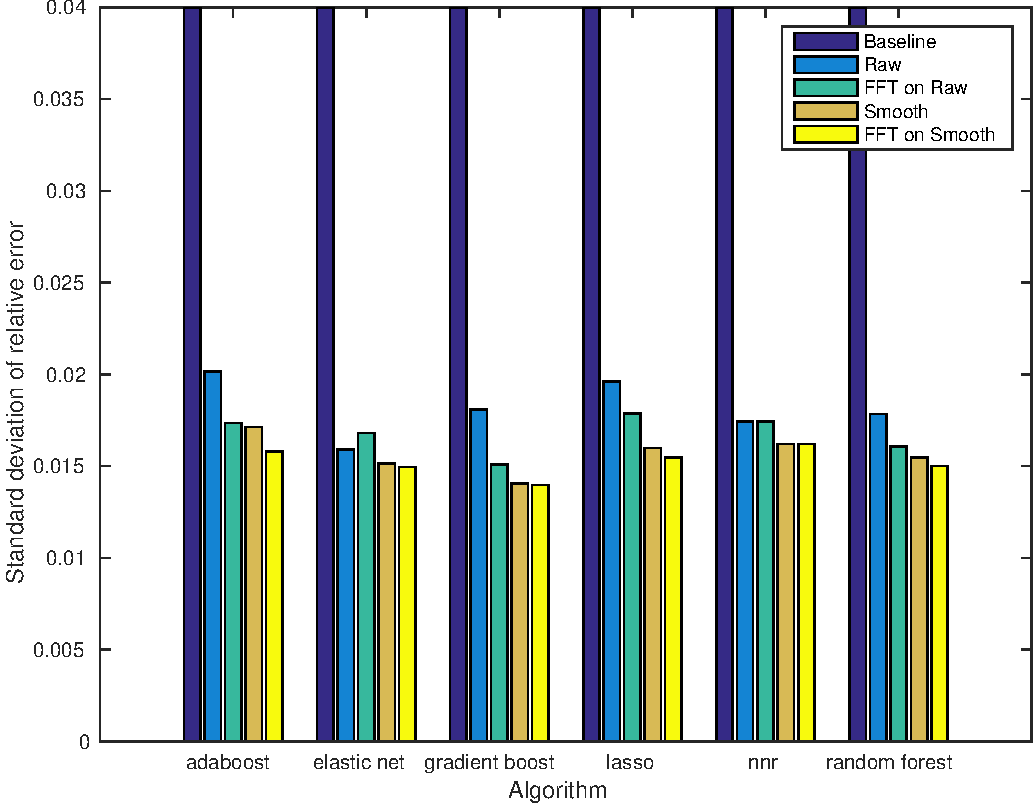
\includegraphics[width=0.45\linewidth]{figures/std_exp4_range50_rates8_pkts16.pdf}
   }
   \caption{Dataset: range 50, rates 8, packets 16}
   \label{fig:exp4}
\end{figure}

\begin{figure}[htpb]
   \centering
   \subfloat[Relative error]{
      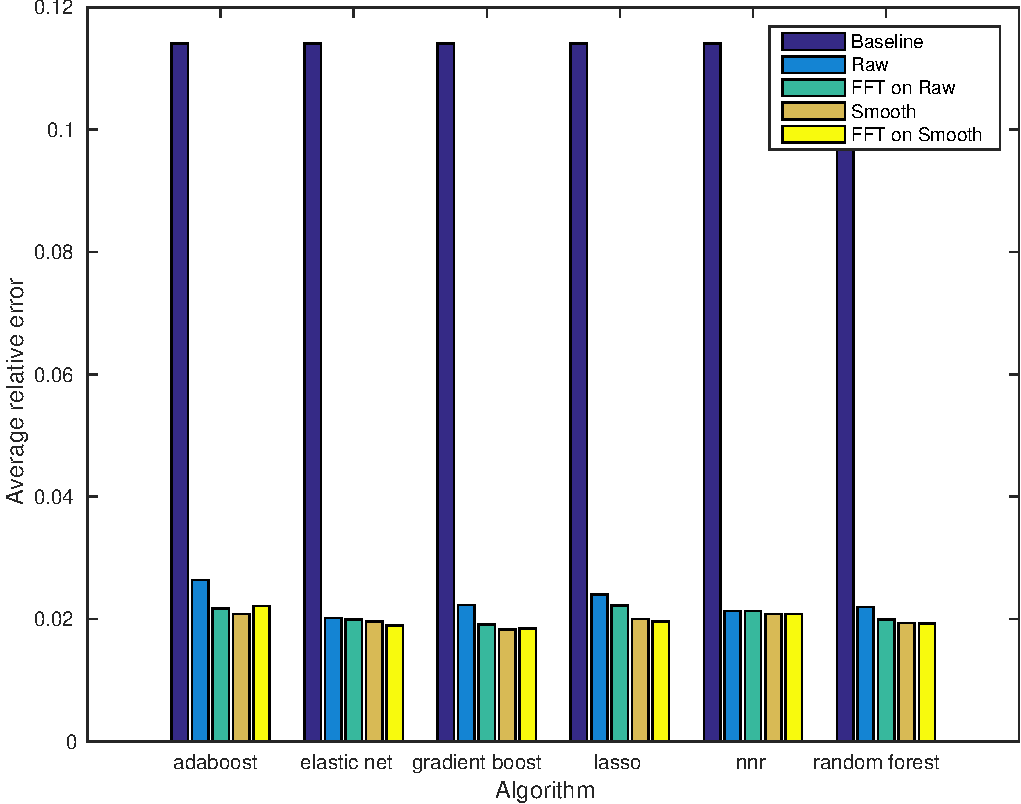
\includegraphics[width=0.45\linewidth]{figures/error_exp5_range50_rates2_pkts64.pdf}
   }
   \quad
   \subfloat[Standard derivation]{
      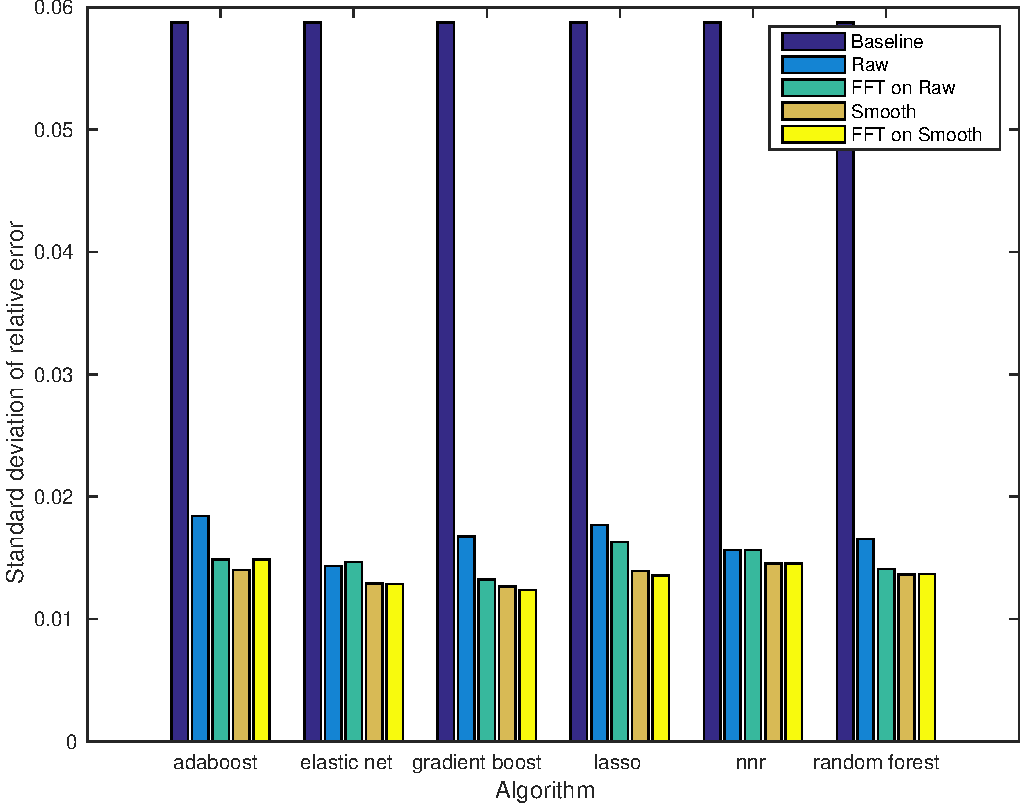
\includegraphics[width=0.45\linewidth]{figures/std_exp5_range50_rates2_pkts64.pdf}
   }
   \caption{Dataset: range 50, rates 2, packets 64}
   \label{fig:exp5}
\end{figure}

\begin{figure}[htpb]
   \centering
   \subfloat[Relative error]{
      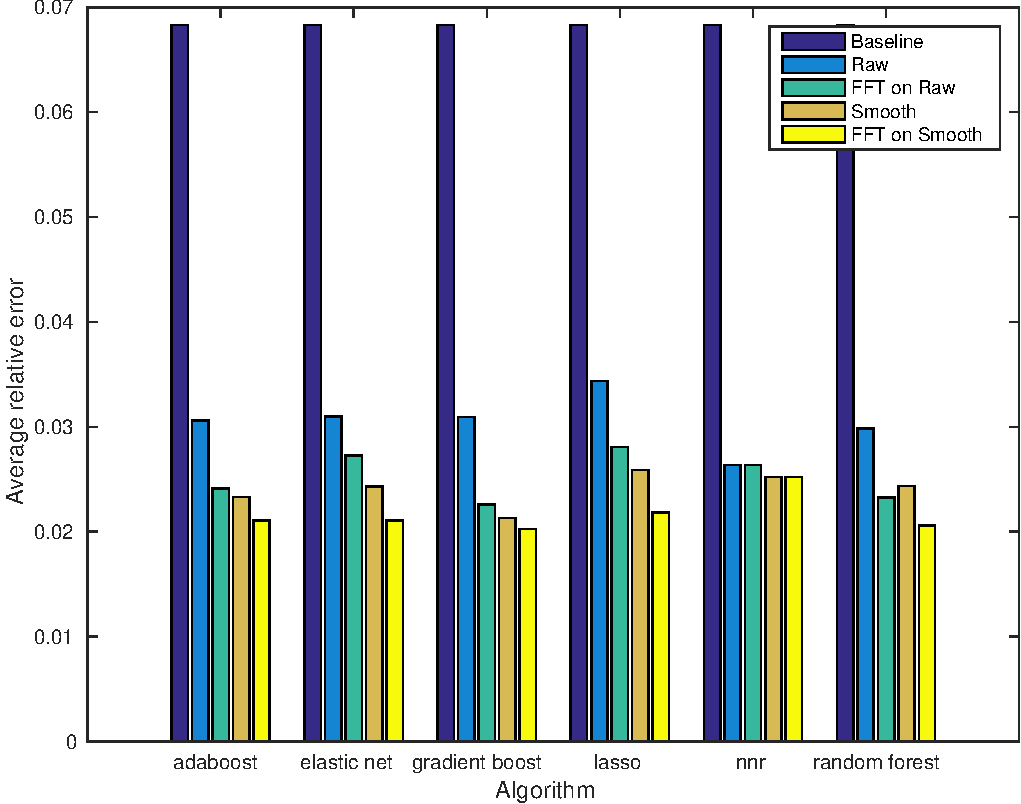
\includegraphics[width=0.45\linewidth]{figures/error_exp6_range50_rates3_pkts43.pdf}
   }
   \quad
   \subfloat[Standard derivation]{
      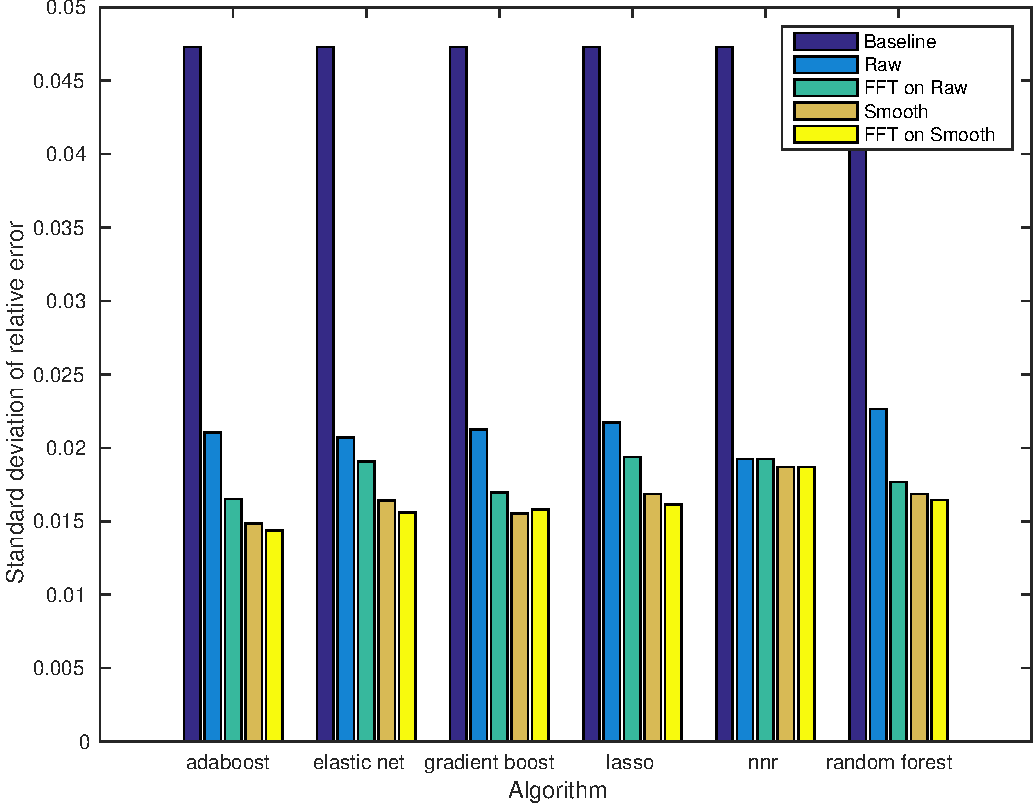
\includegraphics[width=0.45\linewidth]{figures/std_exp6_range50_rates3_pkts43.pdf}
   }
   \caption{Dataset: range 50, rates 3, packets 43}
   \label{fig:exp6}
\end{figure}

\begin{figure}[htpb]
   \centering
   \subfloat[Relative error]{
      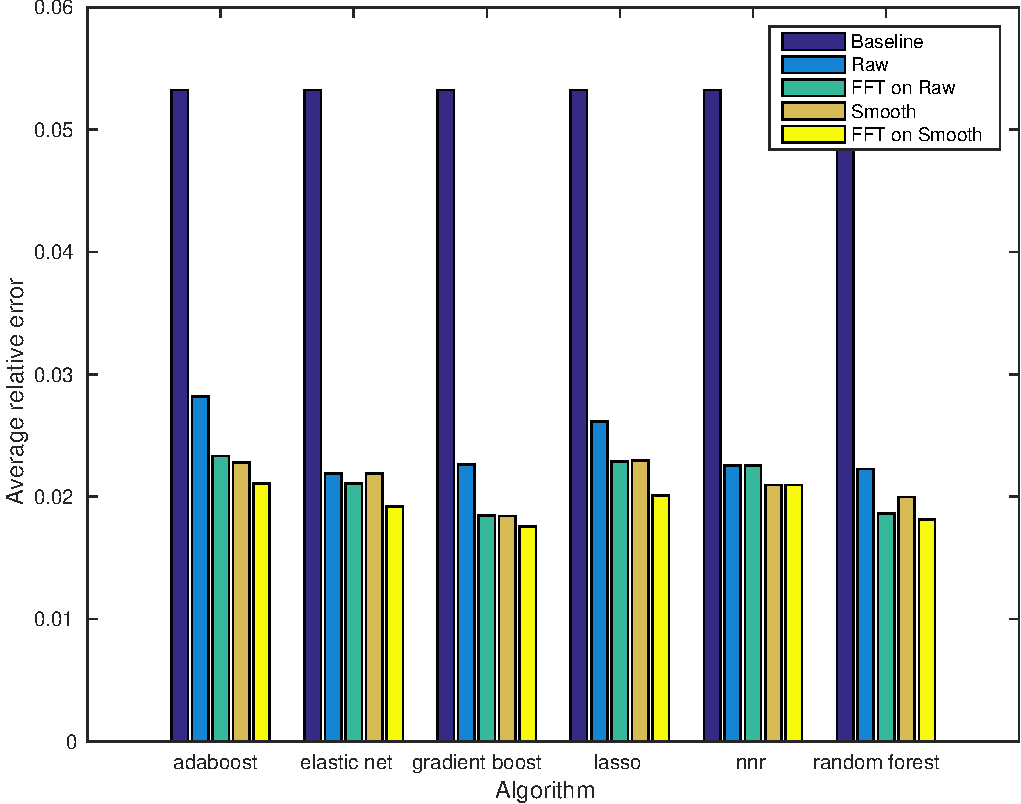
\includegraphics[width=0.45\linewidth]{figures/error_exp7_range50_rates6_pkts21.pdf}
   }
   \quad
   \subfloat[Standard derivation]{
      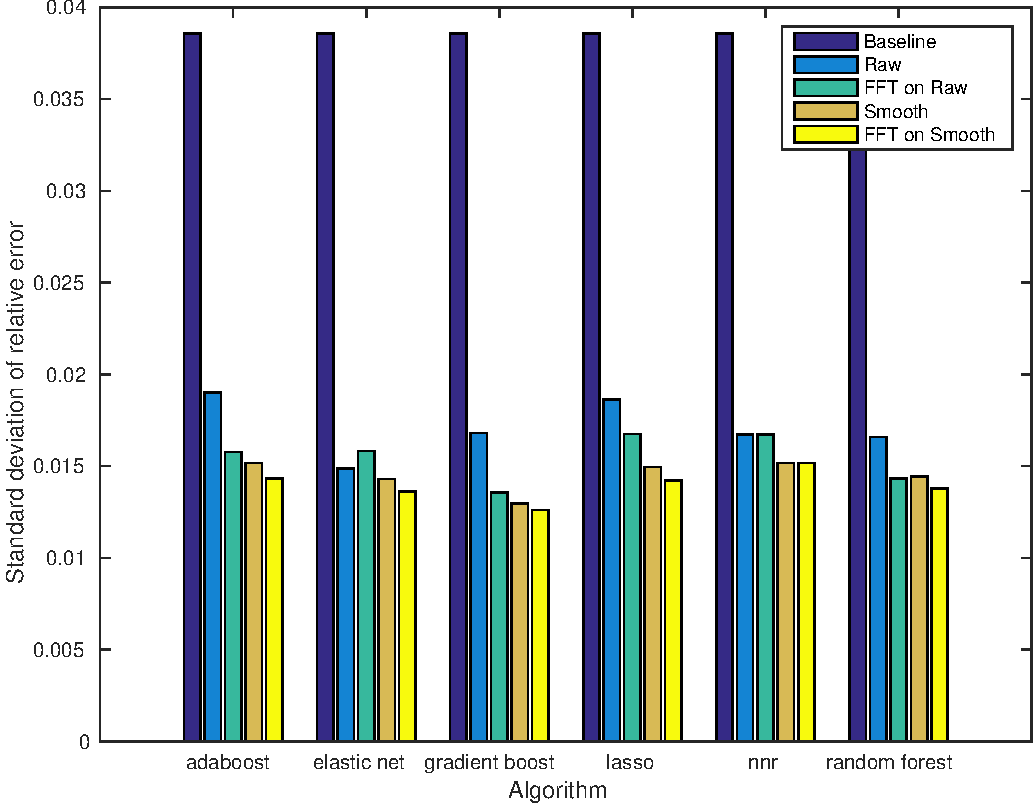
\includegraphics[width=0.45\linewidth]{figures/std_exp7_range50_rates6_pkts21.pdf}
   }
   \caption{Dataset: range 50, rates 6, packets 21}
   \label{fig:exp7}
\end{figure}

\begin{figure}[htpb]
   \centering
   \subfloat[Relative error]{
      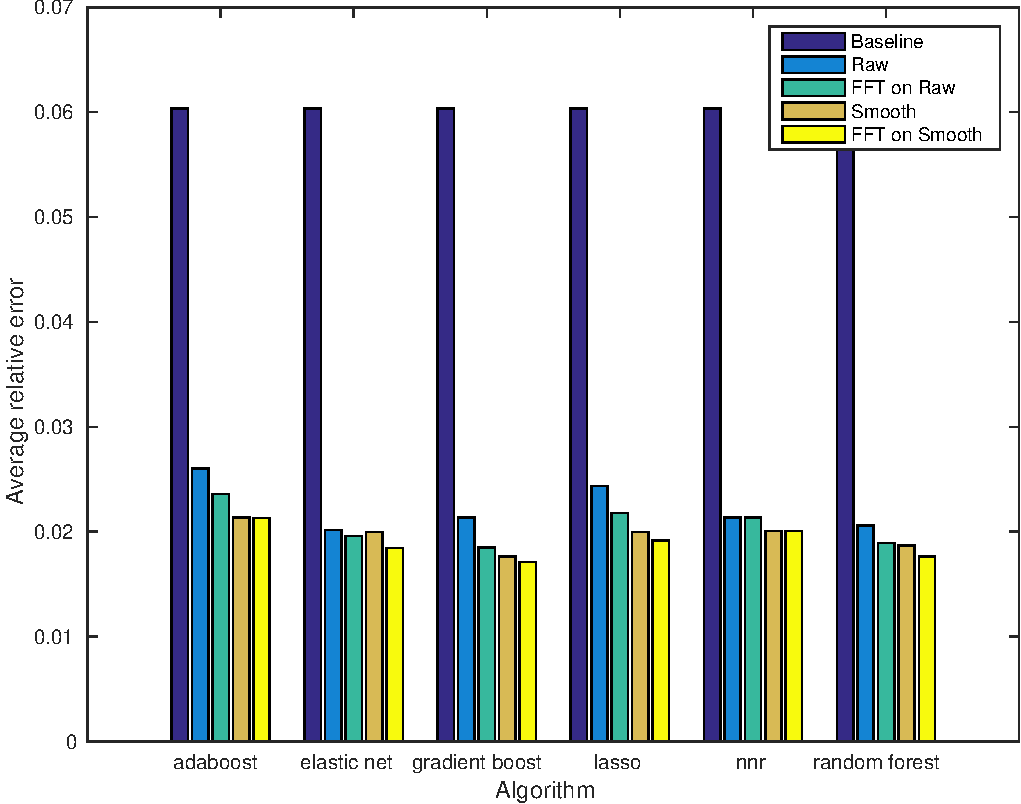
\includegraphics[width=0.45\linewidth]{figures/error_Nov9_range50_rates4_pkts32.pdf}
   }
   \quad
   \subfloat[Standard derivation]{
      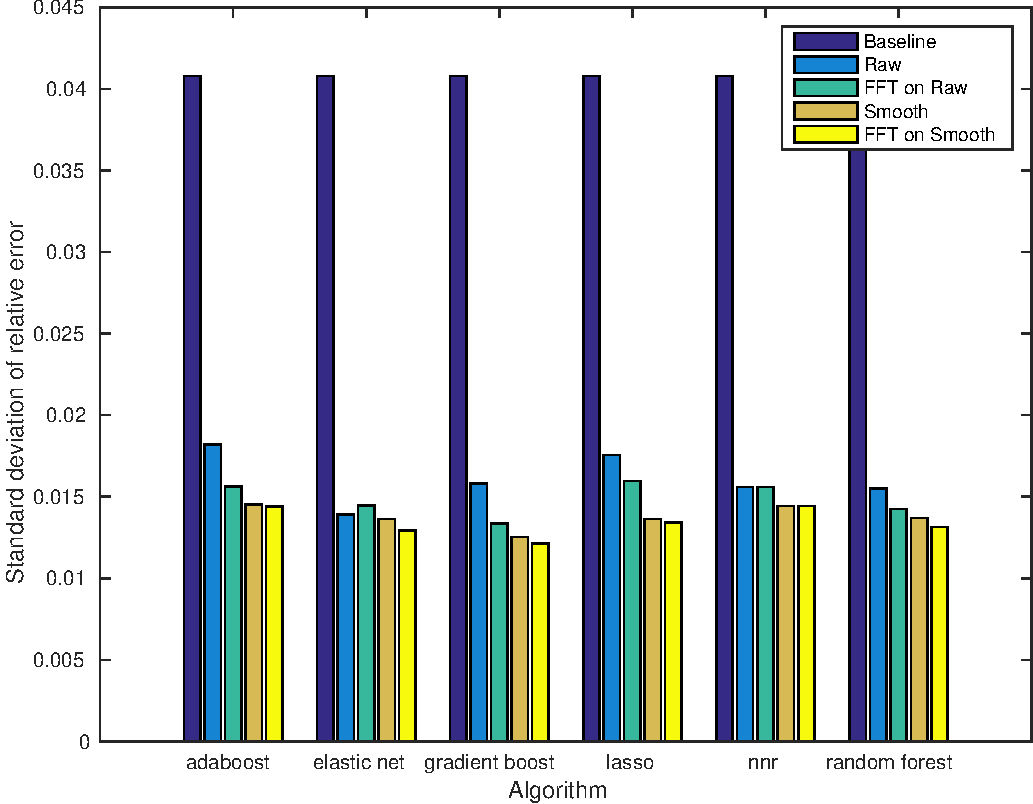
\includegraphics[width=0.45\linewidth]{figures/std_Nov9_range50_rates4_pkts32.pdf}
   }
   \caption{Dataset: range 50, rates 4, packets 32}
   \label{fig:nov9}
\end{figure}
